\subsection{Actual vLLM serving-engine integration}

\label{sec:vllm-system}

We additionally run the adapter inside vLLM 0.31.0's V1 AsyncLLM engine~\cite{Kwon2023vLLM}. The environment uses the CUDA-12.9 vLLM wheel and PyTorch 2.13.0+cu126 on the existing driver. Matching official torchvision/torchaudio CUDA-12.6 wheels and CPU torchcodec remove incidental CUDA-13 multimedia imports; package checks and the actual engine startup both pass.

The serving study uses 1 A40 device and 3 independent process repetitions per policy. GPU 0's sustained occupancy prevented its serving sequence from starting under the idle gate; the two-device operator and PyTorch-model studies remain separate.

The same complete small Qwen3 architecture uses seeded dummy weights, FP16, TP=1, and token-ID inputs. Each policy has its own worker process. All policies retain prefix caching, chunked prefill, the framework's default compilation/graphs, a 4096-token context limit, 16 maximum sequences, and 4096 batched tokens. Prompt lengths are 128 and 2048, concurrency is 1, 8, or 16, and each measured request generates 64 tokens. Two warmup batches precede 128 measured requests per workload. Unique deterministic prefixes prevent cross-request prefix reuse.

The comparison includes the original engine, fixed-native and fixed-compiled adapters, and SCIC. Every candidate passes component checks, and every admitted request's complete generated-token hash matches the original engine at the same seed, workload, and request ID. This verifies generated tokens rather than independently exported full-vocabulary logits. The PyTorch model experiment separately checks full logits.

Across six workloads and 3 paired process repetitions, SCIC's geometric-mean output-throughput ratio is $0.971\times$ relative to the original engine, with a process-bootstrap 95\% interval of $[0.961,0.978]$. This is an aggregate regression under the tested serving configuration; individual workloads differ. The fixed-compiled adapter's corresponding ratio is $0.992\times$. Table~\ref{tab:vllm-serving} reports absolute rates and tail TTFT alongside paired ratios.

\begin{table*}[t]

\centering\small

\caption{Actual vLLM V1 generation, 128 measured requests per process/workload, 64 output tokens per request. Rates are tokens/s and p95 TTFT is in milliseconds; displayed values are medians of per-process values. Ratios and intervals use paired processes. All candidate request token hashes match the original.}

\label{tab:vllm-serving}

\begin{tabular}{@{}rrrrrrr@{}}

\toprule

Input & Conc. & Orig. tok/s & SCIC tok/s & Ratio [95\% CI] & Orig. TTFT$_{95}$ & SCIC TTFT$_{95}$ \\

\midrule

128 & 1 & 538.9 & 531.4 & 0.980 [0.972, 0.986] & 12.45 & 13.78 \\

128 & 8 & 3573.6 & 3185.9 & 0.875 [0.843, 0.892] & 23.58 & 54.74 \\

128 & 16 & 5686.6 & 5382.3 & 1.001 [0.930, 1.053] & 38.62 & 60.55 \\

2048 & 1 & 513.8 & 503.4 & 0.968 [0.912, 1.015] & 14.05 & 15.79 \\

2048 & 8 & 2046.5 & 2148.9 & 1.032 [1.016, 1.053] & 96.49 & 103.95 \\

2048 & 16 & 2953.3 & 2841.1 & 0.977 [0.961, 0.986] & 137.91 & 154.92 \\

\bottomrule

\end{tabular}

\end{table*}

The client benchmark includes IPC, scheduling, KV-cache management, sampling, and streaming. Aggregate throughput also includes deterministic prompt construction; per-request TTFT starts after construction. Tokenizer and HTTP transport are excluded. ITL uses client-observed arrivals, so coalesced tokens share timestamps. Preparation outside regular measurement and any new-signature work inside measured requests retain their actual placement. The available final SCIC worker report records 84 prepared layer/signature entries and 469.467 ms of calibration; early statistics RPC failures are retained and are not replaced by inferred values.

\begin{figure*}[t]

\centering

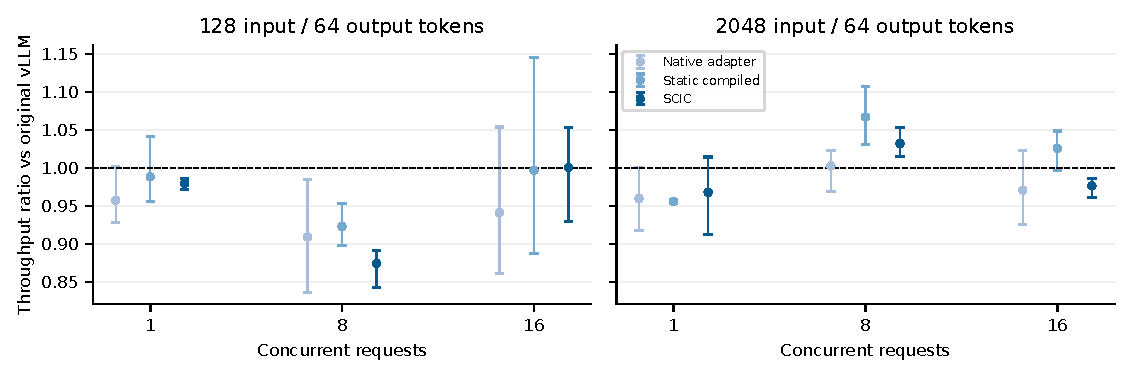
\includegraphics[width=\linewidth]{figures/fig_vllm_serving.pdf}

\caption{Token-validated vLLM serving throughput relative to the original optimized engine. Error bars resample independent process repetitions. The random-weight architecture and fixed batch arrivals do not establish pretrained task quality or production workload behavior.}

\label{fig:vllm-serving}

\end{figure*}
